% Overleaf: select XeLaTeX; this file is self-contained.
\documentclass[11pt,a4paper]{article}
\usepackage[margin=25mm]{geometry}
\usepackage{fontspec}
\setmainfont{texgyrepagella-regular.otf}[BoldFont=texgyrepagella-bold.otf,
  ItalicFont=texgyrepagella-italic.otf,BoldItalicFont=texgyrepagella-bolditalic.otf]
\setsansfont{texgyreheros-regular.otf}[BoldFont=texgyreheros-bold.otf,
  ItalicFont=texgyreheros-italic.otf,BoldItalicFont=texgyreheros-bolditalic.otf]
\setmonofont{lmmono10-regular.otf}[ItalicFont=lmmono10-italic.otf]
\usepackage{amsmath,amssymb,mathtools}
\usepackage{booktabs,tabularx,longtable,array}
\usepackage{enumitem,xcolor,listings}
\usepackage{tikz}
\usetikzlibrary{arrows.meta,positioning}
\usepackage[unicode,colorlinks=true,linkcolor=blue!45!black,urlcolor=blue!55!black,citecolor=blue!45!black]{hyperref}
\usepackage{microtype}
\definecolor{accent}{HTML}{174B70}
\lstset{basicstyle=\ttfamily\footnotesize,breaklines=true,columns=fullflexible,
  keepspaces=true,showstringspaces=false,frame=single,rulecolor=\color{black!15},
  backgroundcolor=\color{black!2},aboveskip=10pt,belowskip=10pt}
\setlist{itemsep=3pt,topsep=5pt}
\setlength{\parskip}{5pt}
\setlength{\parindent}{0pt}
\setlength{\emergencystretch}{3em}
\newcommand{\code}[1]{\nolinkurl{#1}}
\newcommand{\R}{\mathbb{R}}
\newcommand{\E}{\mathbb{E}}
\newcommand{\Lc}{\mathcal{L}}
\newcommand{\impl}{\textbf{Implemented.} }
\newcommand{\plan}{\textbf{Planned experiment.} }
\newcommand{\caution}{\textbf{Interpretation.} }
\title{\textcolor{accent}{Track A: A Scratch Visual Encoder for PushT}\\[5pt]
\large Algorithm, Mathematical Objectives, and Experimental Protocol}
\author{AdaJEPA experimental branch: \texttt{robust-encoder-scratch}}
\date{Implementation snapshot: September 27, 2026}

\begin{document}
\maketitle
\begin{abstract}
This document specifies the implemented Track A experiment in the AdaJEPA repository.
A task-specific vision transformer is trained from random initialization using
masked reconstruction, same-state color translation, and corruption-to-clean
reconstruction. Target rendering colors are supplied to a shared decoder, while
the encoder is encouraged to retain scene information that is stable across
appearance changes. We describe the exact losses, offline four-view dataset,
alternating optimization schedule, frozen linear probes, comparison groups,
logging, and reproducibility constraints. The implementation has passed local
smoke tests; no large-scale training, benchmark improvement, or MPC success gain
has yet been established. Experimental recommendations are explicitly separated
from implemented behavior.
\end{abstract}

\begin{center}
\small
Repository: \url{https://github.com/jinu7513/adajepa}\\
Reviewed base: \code{66c5f18d00cc627ae35b9b183367f7e510972106}\\
Source of truth: \code{conf/tracka.yaml} and \code{tracka/}\newline
Status: implementation and smoke validation; scientific results pending.
\end{center}
\tableofcontents
\newpage

\section{Research question and motivation}
\subsection{Why study the visual encoder?}
PushT planning depends on observing the agent position, block position and
orientation, and target geometry. A change in object color or a moderate blur
can alter image features without changing the underlying scene arrangement.
If the representation moves substantially under such interventions, a predictor
or distance-based planning objective may respond to appearance rather than
task-relevant geometry. Track A tests this potential failure point at the
representation level before modifying planning or dynamics prediction.

The question is: can a PushT-specific encoder trained from scratch preserve
linearly accessible scene geometry while becoming less sensitive to controlled
rendering nuisance and moderate corruption? Better robustness is a hypothesis,
not an assumed consequence of the architecture.

\subsection{Why these design choices?}
\begin{enumerate}
\item \textbf{Scratch initialization} isolates what can be learned from this task's
data. Frozen DINOv2 is an external pretrained reference, not a matched-pretraining control.
\item \textbf{Paired static rerendering} holds scene state approximately fixed while
changing appearance, so aligned image patches have a meaningful correspondence.
\item \textbf{Masked reconstruction} requires the representation to support missing
scene content. The visible-token encoder and lightweight reconstruction decoder
follow the MAE design pattern~\cite{mae}; our task-specific losses and 50\% mask are
implementation choices rather than a reproduction of that paper's full recipe.
\item \textbf{Target-color conditioning} gives the decoder an explicit appearance
input, reducing the need for the encoder to preserve source color for reconstruction.
\item \textbf{A separate corruption objective} avoids requiring reconstruction of
an unpredictable noise realization.
\item \textbf{Frozen clean-trained probes} test whether the same readout continues
to work after visual shift, rather than allowing a new probe to compensate for it.
\end{enumerate}

\subsection{Scope and claim boundaries}
This branch implements encoder pretraining and representation evaluation.
It does not implement Flow-JEPA, flow matching, a new MPC algorithm, test-time
adaptation, or a policy. Earlier last-block/last-two-block and multistep AdaJEPA
adaptation experiments concern a different training/evaluation mechanism.
Here \emph{frozen} means frozen encoder weights during probe fitting, followed by
a fixed probe during shifted evaluation. It does not mean the original paper's
Frozen-versus-AdaJEPA planning comparison.

Matching the existing visual token shape is necessary for interface compatibility,
but a DINO-trained world-model predictor cannot be assumed to understand a newly
trained scratch latent space. End-to-end planning requires a later integration
and training protocol.

\section{Notation and observation model}
Let the available simulator state be
\begin{equation}
s=(a_x,a_y,b_x,b_y,\theta,v_{a,x},v_{a,y})\in\R^7.
\end{equation}
It contains agent and block positions, block angle, and agent velocity.
It does not contain block linear/angular velocity or a complete physics snapshot.
Let the rendering nuisance be
\begin{equation}
\eta=(c_b,c_a,c_g),\qquad c_o\in[0,1]^3,
\end{equation}
where RGB vectors describe the block, agent and goal respectively. If $R$ is the
renderer and $C$ a corruption operator,
\begin{equation}
x=R(s,\eta),\qquad x_{\mathrm{corr}}=C(R(s,\eta),\epsilon).
\end{equation}
Here $\epsilon$ includes random draws; corruption type and strength are recorded
as metadata but never supplied to the encoder or decoder.

The informal goal $E_\theta(x)\approx f(s)$ should be read as stability of
\emph{visually observable} scene information, not invertibility of the full
simulator state. Two states with different velocities may produce the same static
image. Velocity probing is therefore auxiliary, not a decisive test of visual sufficiency.

\begin{table}[htbp]\centering\small
\begin{tabularx}{\linewidth}{lX}
\toprule Symbol & Meaning \\\midrule
$E_\theta,D_\phi$ & Scratch image encoder and shared reconstruction decoder \\
$x_0,x_A,x_B,x_c$ & Clean, two color variants, and corrupted clean image \\
$P=196$, $Q=768$ & Number of patches and RGB pixel values per $16\times16$ patch \\
$d=384$, $d_D=192$ & Encoder and decoder embedding dimensions \\
$M_i,V_i$ & Masked and visible patch indices for sample $i$ \\
$Z_i^u$ & Visible patch representations of view $u$ \\
$B$, $T$ & Batch size and total optimizer-update budget \\
$\lambda_r,\lambda_c,\lambda_g$ & Render, corruption and optional global loss weights \\
\bottomrule
\end{tabularx}
\caption{Core notation. Defaults refer to the checked-in configuration.}
\end{table}

\section{Offline four-view dataset}
\subsection{Exactly four views per accepted state}
For each selected source state, generate
\begin{align}
x_0&=R(\bar{s},\eta_0), & x_A&=R(\bar{s},\eta_A),\\
x_B&=R(\bar{s},\eta_B), & x_c&=C(x_0,\epsilon).
\end{align}
The notation $\bar{s}$ denotes the verified canonical post-reset state; equalities
between separately reset views hold within the configured numerical tolerances.
The corrupted image is computed directly from the stored clean render. It does
not start from a random-color image. Stored images are uint8 PNGs; normalization
is applied in the loader.

The source pool is explicitly selected through \code{dataset.source_path} and
\code{dataset.source_splits}; the latter defaults to \code{[train]}. The generator
reads state tensors and valid sequence lengths, optionally filters shape metadata
to T objects, and rerenders all views. It does not use the planning-target file
\code{val_T/plan_targets.pkl} for pretraining.

\subsection{Canonical state and reset verification}
The current reset path performs one $0.01$-second physics step after assigning
the input state. Let $s^{\rm src}$ be the source state and
\begin{equation}
\bar{s}=\operatorname{Reset}(s^{\rm src},\eta_0),\qquad
s^{q}=\operatorname{Reset}(s^{\rm src},\eta_q).
\end{equation}
Every color view resets from $s^{\rm src}$, not from $\bar{s}$, to avoid an additional
unintended physics advance. Compare each returned state to both $s^{\rm src}$ and
$\bar{s}$. Use coordinate-wise maximum absolute error for each position/velocity
group and the wrapped angular difference
\begin{equation}
\delta_\theta=\operatorname{atan2}\bigl(\sin(\theta-\theta_{\rm ref}),
\cos(\theta-\theta_{\rm ref})\bigr).
\end{equation}
Reject the complete sample if any tolerance fails. Probe labels use $\bar{s}$,
which corresponds to the rendered observation.

\begin{table}[htbp]\centering\small
\begin{tabular}{lrr}
\toprule Field & Source tolerance & Canonical tolerance \\\midrule
Agent position & $5.0$ & $10^{-4}$ \\
Block position & $5.0$ & $10^{-4}$ \\
Block angle (rad) & $0.1$ & $10^{-4}$ \\
Agent velocity & $10^{-3}$ & $10^{-4}$ \\\bottomrule
\end{tabular}
\caption{Current candidate reset tolerances. Positions use simulator coordinates;
velocity uses simulator velocity units. Inspect rejection rates before real training.}
\end{table}

Rejection can bias the accepted data toward slower or non-contact scenes. The
generation report stores per-field maximum errors and rejected counts by split
and trajectory segment; the rejection process must be reported, not hidden by
arbitrarily widening thresholds.

\subsection{Continuous color randomization}
For each object, sample HSV independently before joint rejection:
\begin{equation}
h\sim U(0,1),\quad s_{\rm HSV}\sim U(0.45,0.90),\quad
v_{\rm HSV}\sim U(0.40,0.85).
\end{equation}
Convert to RGB and round to uint8. All rejection distances are Euclidean distances
in the \emph{actual quantized RGB divided by 255}, rather than naive distances in HSV.
The default minimum distances are $0.4$ from white background, $0.3$ between
different objects in one view, and $0.15$ between corresponding objects across views.
Both A and B change all three object colors relative to clean; B also differs from A.
At most 10,000 proposals are attempted before an explicit error.

The default clean RGB values, ordered block/agent/goal, are
$(119,136,153)$, $(65,105,225)$ and $(144,238,144)$. Both pre-quantization sampled
colors and actual renderer RGB are saved. Separate random streams make assignments
independent of scene geometry in the sampling design; a fixed finite dataset can
still exhibit accidental correlations, which probes and held-out trajectories help expose.

\subsection{Continuous corruption strengths}
Corruption types are approximately balanced over selected candidates using a
shuffled schedule. Rejection may slightly alter the accepted distribution.
Each accepted state stores one fixed corruption realization, reused across epochs.
\begin{table}[htbp]\centering\small
\begin{tabularx}{\linewidth}{l l X}
\toprule Type & Training range & Exact semantics \\\midrule
Gaussian & $\sigma\sim U(1,8)$ & Independent zero-mean channel noise in uint8 intensity units; clip to $[0,255]$ and cast to uint8. \\
Salt/pepper & $p\sim U(0.001,0.02)$ & One uniform draw per pixel; probability $p/2$ of white, $p/2$ of black, otherwise unchanged. \\
Blur & $\sigma\sim U(0.3,1.2)$ & Gaussian sigma in image pixels, kernel $\max(3,2\operatorname{round}(3\sigma)+1)$; zero sigma is identity. \\
\bottomrule
\end{tabularx}
\caption{Candidate defaults requiring a visual sanity check on representative source states.}
\end{table}
Canonical salt/pepper probability means expected \emph{selected} pixel fraction;
a pixel that was already white/black may not visibly change. Historical
\code{snp1}/\code{snp5} separately sample salt and pepper positions with replacement
and retain those original semantics. \code{dark} remains available to existing
evaluation code but is not one of Track A's default training corruptions.

The generator first exports deterministic contact sheets, including corruption
strength endpoints and a 50\% spatial mask. Full generation requires
\code{generation.ranges_reviewed=true}. This acknowledges image inspection; it is
not an automated proof that every mask retains every object.

\subsection{Splits, sampling and metadata}
Trajectory IDs are assigned once to approximately 70/15/15\% train/validation/test.
At least one validation and one test trajectory are reserved, so tiny smoke
datasets need not have exact percentages. Default frame stride is five raw frames;
state caps are optional. Sampling and split assignments are stored, never recomputed
from directory ordering. All views of a state stay in the same split.

For valid sequence length $L$ and raw timestep $t$,
\begin{equation}
u=t/\max(L-1,1),\qquad
\operatorname{segment}(u)=
\begin{cases}
\text{early},&0\le u<1/3,\\
\text{middle},&1/3\le u<2/3,\\
\text{late},&2/3\le u\le1.
\end{cases}
\end{equation}
Middle-segment difficulty is an empirical question, not an assumption.
The manifest records source directories, selected IDs/timesteps, seeds, caps,
color/corruption configuration, schema version, metadata hash and code provenance.
Integrity checks verify counts, image paths, verified states and disjoint trajectory sets.

\section{Encoder and shared reconstruction decoder}
\subsection{Visible-only bidirectional encoder}
Normalize input pixels as $\tilde{x}=x/127.5-1$. A $224\times224$ RGB image yields
$P=(224/16)^2=196$ patches, each containing $Q=16^2\cdot3=768$ scalars.
Let $\pi_p(\tilde{x})\in\R^Q$ be patch $p$. Its input token is
\begin{equation}
t_p=W_E\pi_p(\tilde{x})+b_E+e_p.
\end{equation}
At mask ratio $r=0.5$, select $|V|=\lfloor P(1-r)\rfloor=98$ visible patches by a
random permutation. Gather both patch embeddings and their original positional
embeddings using the same \code{ids_keep}. Do not renumber visible spatial positions.

The encoder uses six pre-normalized transformer blocks with six attention heads,
embedding width 384, feed-forward width $4d$, GELU and zero dropout, followed by
LayerNorm. Self-attention is spatially bidirectional. No causal predictor mask is reused.
One mask is shared by clean/A/B during a render update, and by clean/corrupt during
a corruption update. Corresponding latent tokens therefore refer to identical positions.

\subsection{Mask-token restoration}
Project visible latents to width 192, append learned mask tokens, and restore
the original patch order using \code{ids_restore}:
\begin{equation}
H_0=\operatorname{Restore}\left([W_DZ_V+b_D;\,m,\ldots,m]\right)+E_D.
\end{equation}
The shared decoder has two blocks, six heads and a pixel head producing
$\widehat{X}\in\R^{B\times196\times768}$. It predicts every patch, but the main
reconstruction loss is evaluated only on masked positions.

\begin{figure}[htbp]\centering
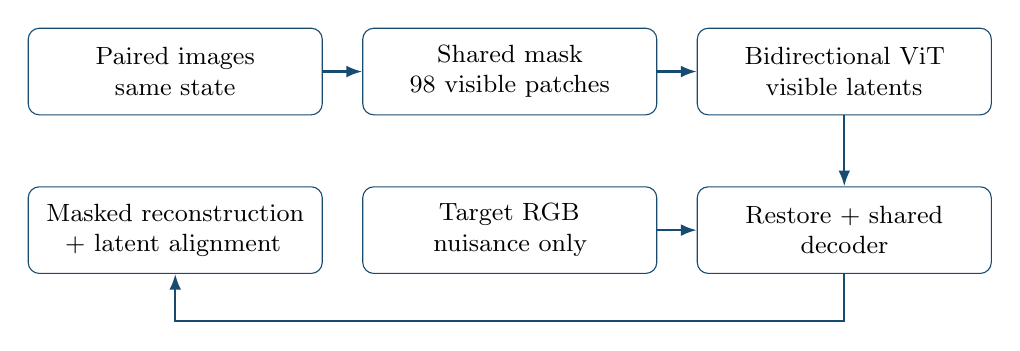
\begin{tikzpicture}[node distance=5mm and 5mm,
 box/.style={draw=accent,rounded corners,align=center,font=\small,minimum height=11mm,text width=35mm},
 arr/.style={-{Latex[length=2mm]},thick,draw=accent}]
\node[box] (views) {Paired images\\same state};
\node[box,right=of views] (mask) {Shared mask\\98 visible patches};
\node[box,right=of mask] (enc) {Bidirectional ViT\\visible latents};
\node[box,below=9mm of enc] (dec) {Restore + shared\\decoder};
\node[box,left=of dec] (eta) {Target RGB\\nuisance only};
\node[box,left=of eta] (loss) {Masked reconstruction\\+ latent alignment};
\draw[arr] (views)--(mask); \draw[arr] (mask)--(enc);
\draw[arr] (enc)--(dec); \draw[arr] (eta)--(dec);
\draw[arr] (dec.south)--++(0,-6mm)-|(loss.south);
\end{tikzpicture}
\caption{Training information flow. Physical-state labels enter only verification and post-training probes.}
\end{figure}

\subsection{Continuous target-RGB conditioning}
For object $o\in\{b,a,g\}$, apply a shared RGB MLP and add a learned type embedding:
\begin{equation}
n_o=f_{\rm RGB}(c_o)+e_{\rm type}(o),\qquad n_o\in\R^{64}.
\end{equation}
The default additive path concatenates in block/agent/goal order:
\begin{equation}
n_{\rm global}=W_n[n_b;n_a;n_g]+b_n\in\R^{192},\qquad
H_{0,p}\leftarrow H_{0,p}+n_{\rm global}.
\end{equation}
The optional cross-attention path projects the three typed tokens to decoder width,
forming $N\in\R^{3\times192}$, and applies
\begin{align}
H'&=H+\operatorname{SA}(\operatorname{LN}(H)),\\
H''&=H'+\operatorname{CA}(\operatorname{LN}(H'),N,N),\\
H_{\rm next}&=H''+\operatorname{MLP}(\operatorname{LN}(H'')).
\end{align}
Additive blocks omit the cross-attention term. The RGB always describes the
\emph{target}, including $\eta_0$ for denoising. Corruption metadata is excluded.

\subsection{Shape contract and optional CLS}
\begin{table}[htbp]\centering\small
\begin{tabular}{ll}
\toprule Tensor & Default shape \\\midrule
Image & $[B,3,224,224]$ \\
Patch pixels & $[B,196,768]$ \\
Full encoder output & $[B,196,384]$ \\
Masked encoder output & $[B,98,384]$ \\
Decoder visible projection & $[B,98,192]$ \\
Restored decoder tokens & $[B,196,192]$ \\
Predicted patch pixels & $[B,196,768]$ \\\bottomrule
\end{tabular}
\caption{Dimensions are configurable; these values describe the default contract.}
\end{table}
Optional CLS processing adds a token internally; the public \code{forward(images)}
still returns patch tokens only. A separate feature API returns CLS when requested.
The optional global path projects CLS to decoder width, broadcasts it over decoder
positions, and reuses the decoder blocks/head to predict the complete target.
It is not a separate independently parameterized decoder network.

\section{Exact training objectives}
\subsection{Masked reconstruction primitive}
Let $m_{ip}=1$ for a masked patch and zero otherwise. For source view $u$ and
target view $v$, define
\begin{equation}\label{eq:rec}
\ell(u\!\to\!v)=
\frac{\sum_{i=1}^B\sum_{p=1}^P m_{ip}
\left[Q^{-1}\sum_{j=1}^Q(\widehat{X}^{u\to v}_{ipj}-X^v_{ipj})^2\right]}
{\sum_{i,p}m_{ip}},
\qquad \widehat{X}^{u\to v}=D_\phi(Z^u,\eta_v).
\end{equation}
By default $X^v$ is the patchified image in $[-1,1]$. With
\code{loss.norm_pix_loss=true}, each target patch is further normalized using
its own pixel mean and population variance plus $10^{-6}$. This is separate
from image normalization. Normalized-pixel predictions do not directly determine
RGB without target statistics; their current preview panels are intentionally blank.

\subsection{Clean MAE baseline}
\begin{equation}
\Lc_{\rm clean}=\ell(0\to0).
\end{equation}
This retains the same conditional decoder architecture but provides the fixed clean
colors. It tests whether ordinary task-specific masked reconstruction is sufficient.

\subsection{Render objective: clean-centered symmetric translation}
For each $q\in\{A,B\}$,
\begin{align}
\Lc_{\rm cross,q}&=\tfrac12\bigl[\ell(0\to q)+\ell(q\to0)\bigr],\\
\Lc_{\rm inv,q}&=\frac{1}{B|V|d}\sum_{i,p\in V_i,k}
\bigl(Z^0_{ipk}-Z^q_{ipk}\bigr)^2.
\end{align}
Average A and B equally within every render update:
\begin{align}
\Lc_{\rm cross}&=\tfrac12(\Lc_{\rm cross,A}+\Lc_{\rm cross,B}),\\
\Lc_{\rm r\text{-}inv}&=\tfrac12(\Lc_{\rm inv,A}+\Lc_{\rm inv,B}),\\
\boxed{\Lc_{\rm render}=\Lc_{\rm cross}+\lambda_r\Lc_{\rm r\text{-}inv}}.
\end{align}
There are four directed reconstructions and three encoded views. Gradients flow
through both sides of latent alignment; there is no frozen teacher or stop-gradient.
The default $\lambda_r=1$ is a starting value, not evidence of an optimal tradeoff.

\subsection{Corruption objective: noisy input, clean target}
\begin{align}
\Lc_{\rm denoise}&=\ell(c\to0),\\
\Lc_{\rm c\text{-}inv}&=\frac{1}{B|V|d}\sum_{i,p\in V_i,k}
\bigl(Z^0_{ipk}-Z^c_{ipk}\bigr)^2,\\
\boxed{\Lc_{\rm corrupt}=\Lc_{\rm denoise}+\lambda_c\Lc_{\rm c\text{-}inv}}.
\end{align}
The default is $\lambda_c=1$. The decoder receives $\eta_0$, not corruption type,
strength or seed. Only masked clean-target pixels are reconstructed: this is not
a full-image denoising loss over every visible pixel. The alignment term additionally
encourages corresponding visible representations to agree.

\subsection{Optional global reconstruction and collapse diagnostics}
For each active directed reconstruction, the CLS path contributes full-patch MSE,
\begin{equation}
\ell_g(u\to v)=\frac{1}{BPQ}\sum_{i,p,j}
\bigl(D_{g,\phi}(z^u_{\rm CLS},\eta_v)_{ipj}-X^v_{ipj}\bigr)^2.
\end{equation}
Average it over the same active directions and add $\lambda_g\Lc_g$ to the selected
objective. CLS, global reconstruction, and $\lambda_g$ are disabled/zero by default.

Latent agreement alone admits constant or low-information solutions. Reconstruction
provides a competing requirement, but it is not a proof against collapse. Monitor
unweighted/weighted losses, latent norms, distances, variance across states and
physical probes. A small distance accompanied by a poor state probe is not success.

\section{Optimization algorithm and budget}
\subsection{Four selectable modes}
\begin{table}[htbp]\centering\small
\begin{tabularx}{\linewidth}{lXrr}
\toprule Mode & Objective & Encoder views/update & Decoder passes/update \\\midrule
\code{clean_mae} & $\Lc_{\rm clean}$ & 1 & 1 \\
\code{render_only} & $\Lc_{\rm render}$ & 3 & 4 \\
\code{corruption_only} & $\Lc_{\rm corrupt}$ & 2 & 1 \\
\code{robust_alternating} & Alternating render/corruption & 3 then 2 & 4 then 1 \\\bottomrule
\end{tabularx}
\caption{Default CLS-disabled computation per sampled state. Counts exclude validation and previews.}
\end{table}
Each run initializes its own encoder/decoder. ``Shared decoder'' means shared
between objectives within a run, not shared weights between experimental runs.

\subsection{Alternating algorithm}
For even total budget $T$, initialize one AdamW optimizer for all trainable parameters.
For $t=0,\ldots,T-1$:
\begin{enumerate}
\item Draw $B$ accepted training-state indices uniformly with replacement.
\item Load the corresponding offline views and target RGB; do not load state labels
into the training batch.
\item Sample a new shared spatial mask for this update.
\item Set $\Lc_t=\Lc_{\rm render}$ if $t$ is even, otherwise $\Lc_{\rm corrupt}$.
\item Zero gradients, compute $\nabla_{\theta,\phi}\Lc_t$, reject non-finite loss/gradient,
clip the global gradient norm to one, and call AdamW once.
\item Set \code{global_step}$=t+1$, record metrics, and periodically validate/save.
\end{enumerate}
One logical cycle consists of two optimizer updates. Clean MAE is not a third default
update. The clean encoding is recomputed at each update; the corrupted batch does
not reuse stale features from the preceding render update. Sequential AdamW updates
with shared moment estimates are not identical to one update on the sum of both losses.

\begin{table}[htbp]\centering\small
\begin{tabular}{lr}
\toprule Parameter & Default \\\midrule
Total optimizer updates & 10,000 \\
Batch size & 16 states \\
AdamW learning rate / weight decay & $10^{-4}$ / $0.05$ \\
Gradient norm cap & $1.0$ \\
Precision / LR schedule & float32 / constant \\
Validation / checkpoint interval & 100 updates / 100 updates \\
Validation cap & 4 batches \\
Image logging interval & 100 updates \\
Scalar logging interval & 10 per-objective updates \\\bottomrule
\end{tabular}
\caption{Defaults, not tuned optima. Alternating scalar cadence samples both objectives.}
\end{table}
The training ``epoch'' field is cumulative sampled states divided by dataset size;
it does not imply a shuffled full pass. Validation currently uses the first capped
set of validation records with fixed mask RNG seed 9871. Its losses are diagnostics,
not an exhaustive evaluation of every held-out state. Use the final fixed-budget
checkpoint for the primary comparison to avoid test-based checkpoint selection.

\subsection{Fairness of the comparison}
Match architecture, mask, optimizer, dataset and total update count across modes.
With $T=10{,}000$, alternating uses 5,000 render plus 5,000 corruption updates.
This is an \emph{update-matched} comparison, not a compute-matched one. With CLS off,
the average encoded/decoded view counts per state draw are 2.5/2.5 for alternating,
versus 1/1 for clean MAE. Log image-pass counts and wall time; a later compute-matched
comparison would be a separate protocol. Timing is per process segment after resume.

\section{Frozen representation evaluation}
\subsection{Physical-state ridge probe}
Freeze the encoder in evaluation mode. Without masking, mean-pool patch tokens:
\begin{equation}
f_i=P^{-1}\sum_{p=1}^{P}E_\theta(x_i)_p\in\R^{384}.
\end{equation}
Targets are computed from canonical rendered state:
\begin{equation}
y_i=(a_x,a_y,b_x,b_y,\cos\theta,\sin\theta,v_{a,x},v_{a,y})\in\R^8.
\end{equation}
Fit feature and target means/stds using clean training observations only, flooring
each standard deviation at $10^{-6}$. For standardized matrices $F,Y$,
\begin{equation}
W_\alpha=\arg\min_W\|FW-Y\|_F^2+\alpha\|W\|_F^2
=(F^\top F+\alpha I)^{-1}F^\top Y.
\end{equation}
The implementation uses the equivalent dual solve when samples are fewer than
feature dimensions. Centering accounts for the intercept. Select
$\alpha\in\{0.001,0.01,0.1,1,10\}$ by clean validation standardized-target MSE.
Freeze this readout and its normalization statistics before any shifted test evaluation.

\subsection{Metrics and their meaning}
For condition $c$ with $n$ test samples, the headline aggregate is
\begin{equation}
\operatorname{SMSE}(c)=\frac{1}{8n}\sum_{i,j}
\left(\frac{\widehat y_{ij}^{c}-y_{ij}}{\sigma^{\rm train}_{y,j}}\right)^2.
\end{equation}
Also report agent-position MSE, block-position MSE and velocity MSE in their original
units, per-target $R^2$, and wrapped angle MAE:
\begin{align}
\widehat\theta_i&=\operatorname{atan2}(\widehat y_{i,\sin},\widehat y_{i,\cos}),\\
\operatorname{MAE}_\theta&=\frac1n\sum_i\left|\operatorname{atan2}
(\sin(\widehat\theta_i-\theta_i),\cos(\widehat\theta_i-\theta_i))\right|.
\end{align}
Angles are reported in radians and degrees. $R^2$ is undefined and stored as null
when the test target has essentially zero variance; negative $R^2$ is possible.
Very small target variance and near-zero predicted sine/cosine pairs require care.

The implemented clean-to-shift degradation is
\begin{equation}
\Delta(c)=\operatorname{SMSE}(c)-\operatorname{SMSE}(0).
\end{equation}
Evaluation latent distance is RMS distance between \emph{mean-pooled full-image}
features. It is distinct from the training loss on aligned visible patch tokens.
Neither raw latent distance nor RGB probe performance alone establishes useful invariance.

\subsection{Test conditions}
\begin{table}[htbp]\centering\small
\begin{tabularx}{\linewidth}{lX}
\toprule Condition & Intervention \\\midrule
default, colorA, colorB & Stored held-out views \\
redBlock, redAgent, redAnchor & Set only the named object's RGB to $(255,0,0)$; anchor means goal marker \\
random\_inside & Fresh random colors under the training sampling bounds \\
random\_outside & Default saturation $[0.91,1]$, value $[0.86,0.95]$; same distance checks \\
Gaussian grid & $\sigma\in\{0,4,8,12\}$ in uint8 units \\
Salt/pepper grid & $p\in\{0,0.01,0.02,0.04\}$ \\
Blur grid & $\sigma\in\{0,0.6,1.2,2\}$ in image pixels \\\bottomrule
\end{tabularx}
\caption{Implemented evaluation protocol, default evaluation seed 100. Zero-strength points are identity controls.}
\end{table}
The default grids span interpolation and stronger extrapolation points. Check
disjointness if training color bounds are changed. Additional evaluation views are
generated separately; they do not alter the four-view training schema. Full/early/
middle/late results use the same clean-trained probe. Rendering is verified against
the saved canonical state. The primary evaluation never refits a probe per shift.

\subsection{Nuisance diagnostics and references}
RGB ridge probes are trained on variable-color A/B views, separately for block,
agent and goal. Clean colors alone would give constant targets and an uninformative
probe. Lower RGB predictability is favorable only if scene information is preserved;
a weak linear probe cannot prove statistical independence.

Corruption-type predictability uses a ridge fit to one-hot labels followed by argmax;
it is not a logistic classifier. Report accuracy, uniform chance and a training-majority
baseline. Strength regression is fit separately for each type to avoid mixing units;
insufficient data is recorded explicitly.

References are random scratch, clean MAE, render-only, corruption-only, alternating,
and frozen pretrained DINOv2~\cite{dinov2}. DINO remains evaluation-only. The existing
wrapper feeds it 196px images with patch14 to yield 196 tokens, whereas scratch uses
224px with patch16. Preserve and record this preprocessing distinction. DINO's external
pretraining data and model history also prevent a strict equal-data comparison.

\section{Experimental design and decision rules}
\subsection{Hypotheses}
\begin{description}
\item[H1: color invariance.] Render-only reduces color-shift degradation relative
to clean MAE without a practically unacceptable loss of clean geometric accuracy.
\item[H2: corruption robustness.] Corruption-only improves corruption curves,
especially within the trained range, relative to clean MAE.
\item[H3: combined utility.] Alternating preserves useful improvements in both
families under a fixed update budget, rather than merely shrinking feature norms.
\item[H4: decoder ablation.] Cross-attention or a CLS global path may change the
geometry/invariance tradeoff; improvement is not presumed.
\end{description}

\subsection{Primary matrix}
\plan Fix one reviewed dataset manifest, split seed, sampling ranges and evaluation
seed. Train the four objectives with seeds $\{0,1,2\}$: 12 independent training runs.
Use additive conditioning, no CLS, mask 0.5, $\lambda_r=\lambda_c=1$, and 10,000 updates.
Pair seeds across objectives for comparison. Evaluate a random encoder and frozen
DINO reference under the same trajectory/probe protocol. The current random-reference
initialization uses \code{evaluation.seed}; rerunning it with another seed also changes
fresh evaluation draws. Keep that seed fixed for the primary reference rather than
pooling incompatible protocols as additional training replicates.

\begin{table}[htbp]\centering\small
\begin{tabularx}{\linewidth}{lX}
\toprule Controlled item & Planned control \\\midrule
Data & Same accepted states, manifest, four stored views and split IDs \\
Initialization & Same training-seed set for the four learned objectives \\
Optimization & Same architecture, batch, LR, optimizer, clipping and update count \\
Checkpoint & Final budget endpoint; no test-based selection \\
Probe & Same mean pooling, clean-only fitting and validation selection grid \\
Test randomness & Fixed evaluation seed and grids across compared learned runs \\
Reporting & Per-condition and per-segment errors, uncertainty across training seeds \\\bottomrule
\end{tabularx}
\caption{Proposed primary comparison. These runs have not yet been performed.}
\end{table}

\subsection{Staged execution and ablations}
\begin{enumerate}
\item Audit real source states and rejection rates; visually review color/corruption
contact sheets before freezing the manifest.
\item Run a two-update smoke job with online W\&B on CIRCE and verify live metrics,
status, local JSONL, checkpoint and reconstruction image.
\item Run clean MAE and alternating for one seed as an engineering pilot. Use it to
detect failures, not to claim a robust scientific result.
\item Execute the preregistered four-objective, three-seed primary matrix.
\item Evaluate all selected checkpoints and the two references using the fixed protocol.
\item Only after the primary matrix, run controlled ablations: zero versus nonzero
invariance weights, additive versus cross-attention, CLS/global off versus on, and
mask ratio. Keep one changed factor per comparison.
\end{enumerate}
Suggested exploratory grids are $\lambda\in\{0,0.1,1\}$ and mask ratio
$r\in\{0.25,0.5,0.75\}$; these are recommendations, not executed or tuned values.
With separate render/corruption weights, vary one while fixing the other before
attempting a larger interaction study. Record every attempted setting, not only winners.

\subsection{What would support or weaken the claim?}
\plan Report clean errors alongside every shifted error. A method that lowers
shift degradation by making clean performance worse is not necessarily useful.
Before final testing, choose a domain-meaningful acceptable clean geometric-error
increase using training/validation evidence and record it. No numerical acceptance
threshold has yet been established in this implementation.

Evidence favoring the approach would combine stable clean position/angle accuracy,
smaller errors under both color and corruption interventions, and consistency across
training seeds. Improvement only on trained corruption strengths suggests interpolation
robustness, not unrestricted generalization. Poor RGB predictability with poor geometry
suggests information loss. Good reconstruction with poor probes suggests that pixel
reconstruction alone has not established a useful representation.

\subsection{Statistical reporting}
The current aggregation script reports mean and sample standard deviation across
distinct training seeds, not a confidence interval. With $K$ runs,
\begin{equation}
\bar m=K^{-1}\sum_km_k,\qquad
s_m=\sqrt{\frac{\sum_k(m_k-\bar m)^2}{K-1}}.
\end{equation}
Three seeds provide a first stability check, not strong statistical power. Frames
within a trajectory are correlated. Current per-run metrics are frame-weighted;
longer accepted trajectories can contribute more. A future trajectory-balanced or
trajectory-bootstrap analysis should resample whole trajectories, not independent
frames, and would require retaining/exporting per-sample predictions beyond the
current aggregate reports. Do not label existing SD bars as confidence intervals.

\section{Logging, reproducibility and run management}
\impl W\&B project defaults to \code{adajepa_trackA}. Names include objective,
conditioning, mask ratio and seed. Training curves use \code{train/global_step}.
Local JSONL is flushed before W\&B logging, so scalar records survive service
failure. Config, dataset manifest hash, source hash, git SHA and dirty state accompany
the run. Per-condition probe tables, color-shift bars and separate strength curves
are also recorded; all have local counterparts.

Monitor \code{render/cross_mae}, \code{render/invariance}, their weighted form,
corruption denoising/invariance counterparts, \code{clean/mae}, total/global losses,
latent norms/variance/distances, gradient norm, LR, sample count, image-pass counts,
and elapsed time. Validation diagnostics use separate keys. Training epoch, optimizer
step and MPC step are different concepts; this branch produces no MPC success-rate curve.

Checkpoint dictionaries save encoder, shared decoder and optimizer states; update,
cycle and sample counters; next objective; RNG states; resolved config; manifest/schema
identity; git/source provenance; output path and W\&B run ID. Float32 constant-LR
training has no AMP scaler or scheduler to resume. Online resume requires the original
project/entity and run ID; incompatible config/manifest or stale checkpoints are rejected.
Offline resume starts a new offline segment with continuous local optimizer steps.

Normal and exception exits finalize W\&B with distinct status, and Python exceptions
are preserved locally. SIGKILL or power loss cannot run finalization. A recovery CLI
replays local metrics/tables/charts into a clearly named new run. Writable local
cache/staging defaults prevent artifact uploads from depending on a writable home
cache. Offline serialization has been verified; authenticated cloud delivery remains
to be checked on CIRCE.

\section{Implementation evidence and limitations}
The local suite passed 24 tests under Python 3.11.14, PyTorch 2.3.0, torchvision
0.18.0, NumPy 1.26.4, Hydra 1.3.2, W\&B 0.22.3 and pymunk 6.6.0. Tests cover actual
PushT rerendering, state/mask integrity, all objectives and conditioning modes,
backpropagation, CLS compatibility, CPU resume equality, probe fitting and offline
W\&B chart recovery. Python 3.9 syntax was checked; its actual runtime, CUDA, real
CIRCE training data and DINO weight loading were not tested locally.

\begin{enumerate}
\item The state model is incomplete and static images do not identify every state component.
\item Reconstruction and MSE alignment do not guarantee causal disentanglement or prevent collapse.
\item The same finite offline noise/color samples recur throughout training.
\item Reset rejection and accepted-trajectory lengths can change the evaluated population.
\item Linear-probe success measures accessible information, not policy success.
\item The current strength diagnostics concern each corruption separately. Joint color-plus-noise
generalization is a future experiment, not an implemented benchmark result.
\item Default loss weights, corruption ranges and sample budget require empirical validation.
\item Shape compatibility with AdaJEPA does not establish latent compatibility with existing checkpoints.
\end{enumerate}
No success-rate values from previous planning runs should be presented as results
of this new encoder experiment. The next defensible output is a completed, reproducible
representation comparison with clearly labeled experimental uncertainty.

\appendix
\section{Runnable command sequence}
These are Bash commands in the repository on CIRCE. Replace the source/checkpoint
paths with actual paths. They are derived from the implemented Hydra config.
\begin{lstlisting}
SOURCE=/absolute/path/to/pushT_dataset
PAIRS="$PWD/data/tracka_pairs"

python generate_pusht_pairs.py --config-name tracka \
  dataset.source_path="$SOURCE" dataset.output_path="$PAIRS" \
  generation.preview_only=true

# After inspecting the exported contact sheets:
python generate_pusht_pairs.py --config-name tracka \
  dataset.source_path="$SOURCE" dataset.output_path="$PAIRS" \
  generation.preview_only=false generation.ranges_reviewed=true

# Engineering smoke run; no full-scale training:
python train_encoder.py --config-name tracka \
  dataset.output_path="$PAIRS" training.objective=robust_alternating \
  training.total_optimizer_updates=2 training.batch_size=2 \
  logging.log_every=1

# Planned primary matrix, executed sequentially when resources are allocated:
for SEED in 0 1 2; do
  for MODE in clean_mae render_only corruption_only robust_alternating; do
    python train_encoder.py --config-name tracka \
      dataset.output_path="$PAIRS" training.objective="$MODE" \
      training.seed="$SEED" logging.group="trackA-seed${SEED}"
  done
done
\end{lstlisting}
For each printed run directory, evaluate its final checkpoint and retain the results:
\begin{lstlisting}
python eval_encoder_probes.py --config-name tracka \
  dataset.output_path="$PAIRS" evaluation.encoder=checkpoint \
  evaluation.checkpoint=/absolute/path/to/run/checkpoint_latest.pt

python eval_encoder_probes.py --config-name tracka \
  dataset.output_path="$PAIRS" evaluation.encoder=random

python eval_encoder_probes.py --config-name tracka \
  dataset.output_path="$PAIRS" evaluation.encoder=dino

python aggregate_tracka_results.py \
  /absolute/path/to/probe_clean /absolute/path/to/probe_robust \
  --output-dir "$PWD/tracka_outputs/comparison"

python recover_tracka_wandb.py /absolute/path/to/run
\end{lstlisting}
Use \code{logging.mode=offline} when cloud access is unavailable. Resume requires
the original nondefault model/loss/training settings along with
\code{training.resume=/absolute/path/to/checkpoint_latest.pt} and a larger total budget.
Dataset source files include \code{states.pth}, \code{velocities.pth} when needed,
\code{seq_lengths.pkl}, and optional \code{shapes.pkl}. Keep any real large-scale
launch within the cluster's allocated resources; no scheduler resource request is
invented by these commands.

\section{Code-to-method map}
\begin{longtable}{p{0.43\linewidth}p{0.49\linewidth}}
\toprule File & Method responsibility \\\midrule\endhead
\code{conf/tracka.yaml} & Defaults and all experiment switches \\
\code{tracka/data.py} & Rerendering, rejection, four-view records, manifests and loading \\
\code{tracka/model.py} & Encoder, shared decoder, mask restoration and exact losses \\
\code{tracka/train.py} & Sampling, objective schedule, optimization and resume \\
\code{tracka/probes.py} & Clean-trained ridge probes, references and shifted evaluation \\
\code{tracka/logging.py} & Durable local logs and W\&B lifecycle/charts \\
\code{planning/image_corruption.py} & Canonical and backward-compatible corruption functions \\
\code{aggregate_tracka_results.py} & Protocol-compatible grouping, CSV and seed SD figure \\
\code{tests/test_tracka.py} & Smoke and regression evidence \\
\code{docs/tracka_validation.md} & Actual validation environment and limitations \\\bottomrule
\end{longtable}

\begin{thebibliography}{9}
\bibitem{mae} K. He, X. Chen, S. Xie, Y. Li, P. Doll\'ar, and R. Girshick.
\emph{Masked Autoencoders Are Scalable Vision Learners}. arXiv:2111.06377, 2021.
\url{https://arxiv.org/abs/2111.06377}.
\bibitem{dinov2} M. Oquab et al.
\emph{DINOv2: Learning Robust Visual Features without Supervision}.
arXiv:2304.07193, 2023.
\url{https://arxiv.org/abs/2304.07193}.
\end{thebibliography}
\end{document}
